\documentclass[letterpaper, 11pt]{extarticle}

\input{preamble}
\input{format}
\input{commands}

\begin{document}

\begin{Large}
    \textsf{\textbf{CS361 - HW1}}
\end{Large}

\vspace{1ex}

\textsf{\textbf{Student:}} \text{Shrey Poshiya}\\

Github Link: https://github.com/sposhiy33/CS361HW1

\vspace{2ex}


% Problem 1, Sorting lol
\begin{problem}{}{problem-label}

    Sort the following functions based on their asymptotic growth rate with brief explanations. Example: $f1 < f2 = f3 < f4$
    
    \[
    10^{(-10)}, \ 10^{(10)}, \ n^2, \ (\log_2 n)^2, \ 2^n, \ 3^n, \ n \log_2 n, \ \log_2 n, \ \log_3 n, \ 2^{(\log_2 n)},
    \]
    \[
    \sqrt{n}, \ (\sqrt{2})^{\log_2 n}, \ (\log_2 n)^{(\log_2 n)}, \ \log_2(\sqrt{n}), \ \log_2(\log_2 n), \ n!
    \]

\end{problem}

\[ 
10^{(-10)} = 10^{(10)} <
\log_2(\log_2 n) <
\log_3 n = 
\log_2(\sqrt{n}) = \log_2 n <
(\log_2 n)^2 <
\sqrt{n} = 
\ldots \]

\[ \ldots
(\sqrt{2})^{(\log_2 n)} <
2^{(\log_2 n)} <
n \log_2 n <
n^2 <
(\log_2 n)^{(\log_2 n)} <
2^n <
3^n <
n! \]

Generally, it is known that: logarithm $\leq$ linear $\leq$ quadratic $\leq$ exponential $\leq$ factorial (as $n \rightarrow \infty$) ... my inequality follows this pattern

Some simplifications:
\begin{itemize}
    \item $ 10^{(-10)} = 10^{(10)} $  are constant so they will have $O(1)$
    
    \item $2^{(\log_2 n)} = n$ ... this is linear time complexity $O(n)$
    
    \item  $\sqrt{2}^{(\log_2 n)} = 2^{\frac{1}{2}\log_2 n} = n^{\frac{1}{2}} = \sqrt{n}$ ... this will have $O(\sqrt{n})$
    
    \item $\log_2(\sqrt{n}) = \frac{1}{2}\log_2(n)$, so this reduces down to $O(\log_2 n)$
    
\end{itemize}

Specific comparisons I made:
\begin{itemize}

    \item Compare $\log_3 n$ and $\log_2 n$.

    \[ \lim_{n \rightarrow \infty} \frac{\log_3 n}{log_2 n} = \lim_{n \rightarrow \infty} [\frac{\frac{1}{n \ln{3}}}{\frac{1}{n \ln{2}}} = \frac{n \ln{2}}{n \ln{3}}  = \frac{\ln{2}}{\ln{3}}] = \frac{\ln{2}}{\ln{3}} \]

    Since the result of the limit is a finite, positive constant, the asymptomatic behavior of the two functions are similar.

    \item Compare $\sqrt{n}$ and $\log_2 n$.
    \[ \lim_{n \rightarrow \infty} \frac{\sqrt{n}}{\log_2 n}\ = \lim_{n \rightarrow \infty} [ \frac{\frac{1}{2 \sqrt{n}}}{\frac{1}{n \ln{2}}} = \frac{n \ln{2}}{2 \sqrt{n}} = \frac{\sqrt{n} \ln{2}}{2}] = \infty \]
    By the limit theorem, $\sqrt{n}$ grows faster. Therefore logarithm $\leq$ square root.

    \item Since $\log_2 n \leq \sqrt{n}$, it follows that $(\log_2 n)^2 \leq n$. Therefore, we can say  \\ $(\log_2 n)^2  \leq 2^{(\log_2 n)}$

    \item Compare $\sqrt{n}$ and $(\log_2 n)^2$

    \[\lim_{n \rightarrow \infty} \frac{\sqrt{n}}{(\log_2 n)^2} = \lim_{n \rightarrow \infty} [\frac{\frac{1}{2 \sqrt{n}}}{\frac{2 \log_2 n}{n \ln{2}}} = \frac{n \ln{2}}{4 (\sqrt{n})(\log_2 n)} = \frac{\sqrt{n} \ln{2}}{4 \log_2 n}] = \lim_{n \rightarrow \infty} [ \frac{\frac{\ln{2}}{\sqrt{n}}}{\frac{4}{n \ln{2}}} = \frac{n(\ln{2})^2}{4 \sqrt{n}} = \frac{\sqrt{n} (\ln{2})^2}{4}] =  \infty \]

    By the limit theorem, $\sqrt{n}$ grows faster than $(\log_2 n)^2$
    \item Since it is known that $\log_2 n \leq n$, we can conclude that $\log_2(\log_2 n) \leq \log_2 n$. 
    % So to find the final position of $\log_2(\log_2 n)$, compare it with $\log_3 n$.

    % \[
    % \lim_{n \rightarrow \infty} \frac{\log_3 n}{(\log_2 (\log_2 n))} = \lim_{n \rightarrow \infty} [ \frac{\frac{1}{n \ln{3}}}{\frac{1}{(\log_2 n) \ln{2}}  * \frac{1}{n\ln(2)}} =
    % \frac{n (\ln{2})^2 (\log_2 n)}{n\ln{3}} = \frac{ (\ln{2})^2 (\log_2 n)}{\ln{3}} ] = \infty
    % \]

    % By the limit theorem, $\log_3 n$ grows faster.

    \item Now compare $(\log_2 n)^{\log_2 n}$ with all terms greater than $2^{(\log_2n)}$, to find where $(\log_2 n)^{\log_2 n}$ fits in:

    \begin{itemize}
        \item comparing $(\log_2 n)^{\log_2 n}$ and $n^2$. Since logarithms preserve inequality, taking the logarithm of both functions will allow us to examine the relationship more simply:

        $$\log_2((\log_2 n)^{\log_2 n}) = (\log_2 n) (\log_2(\log_2 n))$$
        $$\log_2(n^2) = 2\log_2 n$$

        Since $(\log_2(\log_2 n))$ is larger than $2$ as n grows, we can confidently say that $(\log_2 n)^{\log_2 n} > n^2$. Take the logarithm of both sides and compare the resulting values:

        \item By similar strategy, we can compare $(\log_2 n)^{\log_2 n}$ and $2^n$

        $$\log_2((\log_2 n)^{\log_2 n}) = (\log_2 n) (\log_2(\log_2 n))$$
        $$\log_2(2^n) = n \log_2(2) = n$$

        $(\log_2 n) (\log_2(\log_2 n))$ is the product of two log terms, which will grow slower than a linear term, so $2^n$ is larger.
        
    \end{itemize}
    
\end{itemize}





\begin{problem}{}{problem-label-2}
    Show that:
    \begin{itemize}
        \item $\log_{2}(n!) = \Omega(1)$ and $\log_{2}(n!) = O(n \log_{2}n)$
        \item $3n^{\sqrt{n}} = \Theta(2^{(\sqrt{n} \log_{2}n)})$
    \end{itemize}
\end{problem}

\begin{itemize}
    \item $\log_{2}(n!) = \Omega(1)$: This is true if: $\exists \ (c_0, N_0) > 0 \ \text{such that} \log_2(n!) \geq c_o * 1 \ \ \forall n> N_0$

        \[ 
        \text{Simplify the expression by taking each side to base 2:} \ \ n! \geq 2^{c_0}
        \]
        \[
        \text{Choose} \ \ c_0=1,\ \text{then choosing} \ \ N_0 = 2 \ \ \text{will satisfy the above inequality}
        \]


    \item $\log_{2}(n!) = O(n \log_{2}n)$: \\ $\exists \ (c_0, N_0) > 0 \ \text{such that} \log_2(n!) \leq c_o * n \log_{2}n \ \ \forall n>N_0$ 

        \[ \text{Simplify the expression by taking each side to base 2:} \ \ n! \leq 2^{c_0 * n \log_2 n} \]
        \[ \text{now since } 2^{c_0 * n \log_2 n} = (2^{\log_2 n})^{c_0 * n} = n^{c_0 * n}, \text{ the inequality becomes}\]
        \[ n! \geq n^{c_0 * n} \]
        \[ \text{let $c_0 = 1$, then find $N_0$ such that $n! \geq n^{n} \ \ \forall n > N_0$ }\]
        \[ \text{let $N_0 \geq 2$ and the above inequality is satisfied} \]
    
    \item $3n^{\sqrt{n}} = \Theta(2^{(\sqrt{n} \log_{2}n)})$: \\ $\exists \ (c_1, c_2, N_0) >0 \ \text{such that} \ c_1 * 2^{(\sqrt{n} \log_{2}n)} \leq 3n^{\sqrt{n}} \leq c_2 * 2^{(\sqrt{n} \log_{2}n)}$ 

        \[ \text{First, simplify} \ 2^{(\sqrt{n} \log_{2}n)} =  (2^{(\log_{2}n)})^{\sqrt{n}} = n^{\sqrt{n}} \]
        \[ \text{The inequality now becomes} \ \  c_1 * n^{\sqrt{n}} \leq 3*n^{\sqrt{n}} \leq c_2 * n^{\sqrt{n}} \]
        \[ \text{Therefore, we can choose  } 0 < c_1 \leq 3 \ \ \text{and } 3 \leq c_2 \text{ and the inequality will be satisfied for all N $>$ 0}\]
    
\end{itemize}

\begin{problem}{}{problem-3}
    Give asymptotic bounds for $T(n)$ in each of the following recurrences. Assume that $T(n)$ is small for sufficiently small $n$. Make your bounds as tight as possible and justify your answer.
    \begin{itemize}
        \item $T(n) = 3T(n/2) + n$
        \item $T(n) = 8T(n/2) + n^2$
    \end{itemize}
\end{problem}

Both recurrence relations are in the current form to use Master theorem, meaning that we can get exact-bound cases for both relations:


\begin{itemize}
    \item $T(n) = 3T\left(\frac{n}{2}\right) + n$

            \[a = 3, \ b = 2, \ f(n) = n \rightarrow k = 1, p = 0 \]
            \[ \text{since} \log_2(3) > 1 = k, \ \ \Theta\left(n^{\log_2(3)}\right) \]

    \item  $T(n) = 8T\left(\frac{n}{2}\right) + n^2$

            \[ a = 8, \ b = 2, \ f(n) = n^2 \rightarrow k = 2, \quad p = 0 \]
            
            \[ \text{Note that, } \log_2(8) = 3. \text{ Since } 3 > 2, \text{it follows } \Theta(n^3) \]
    
\end{itemize}


\begin{problem}{}{problem-4}
    Given Method-1 and Method-2 discussed in class, plot time graph using Matplotlib or any programming language of your choice and discuss the results. Also plot $n!$ and $2^n$ in a similar way and discuss the results. Prove the relationship between the two using limit theorem.
\end{problem}

\begin{figure}[H]
    \centering
    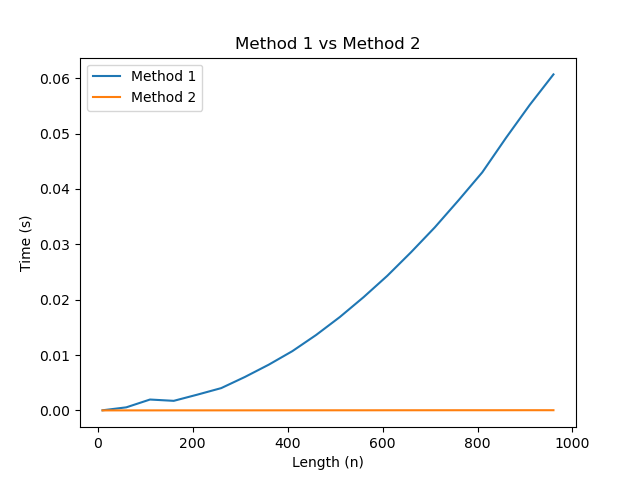
\includegraphics[width=0.75\linewidth]{assets_HW1/P4-1.png}
    \caption{Empirical results of execution time of Method-1 and Method-2}
    \label{fig:p4-1}
\end{figure}

Comparing method-1 and method-2, we see that method-1 has a higher empirical execution relative to method-2 as $n \rightarrow \infty$. This is expected given the nested for-loops in method-1, meaning that the time complexity is $O(n^2)$. The single for-loop in method-2 indicates that it will have a linear time complexity, $O(n)$. We see this broadly reflected in Figure 1, with method-1 execration following a quadratic pattern while method-2 stays linear.

\begin{figure}[H]
    \centering
    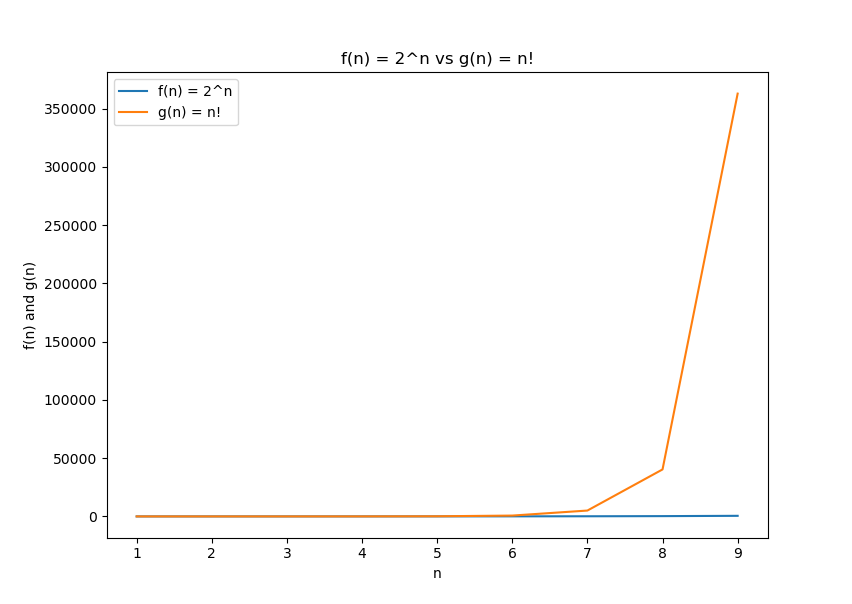
\includegraphics[width=0.75\linewidth]{assets_HW1/P4-2.png}
    \caption{Comparison between $n!$ and $2^n$ for values of $n$ from 1-9} 
    \label{fig:p4-2}
\end{figure}

In Figure 2, I plot the values of the function as the n is varied. We see that $n!$ grows much faster than the exponential function, $2^n$ as $n \rightarrow \infty$

\[ \lim_{n \rightarrow \infty} \frac{2^n}{n!} \]

Since this factorial term is irreducible using L'hopital's rule, the ratio test can be used to evaluate the convergence of the above limit.

According to the ratio test if $\lim_{n \rightarrow \infty} \frac{a_{n+1}}{a_n}$ convergences to a value less than $1$, then 
$\lim_{n \rightarrow \infty} a_n =0$

\[ \lim_{n \rightarrow \infty} \frac{a_{n+1}}{a_n} = \lim_{n \rightarrow \infty} [\frac{\frac{2^{n+1}}{(n+1)!}}{\frac{2^n}{n!}} = \frac{2^{n+1}}{2^n}\frac{n!}{(n+1)!} = 2n] = 0\]

Therefore, $$\lim_{n \rightarrow \infty} \frac{2^n}{n!} = 0$$

By the Limit Theorem, this means that $$2^n = O(n!)$$

This result agrees with the results from Figure 2.

\begin{problem}{}{problem-5}
    Implement Insertion sort in reverse and show a working example on array of length 5 (not sorted).
\end{problem}

\begin{lstlisting}[language=Python, basicstyle={\small\ttfamily}]
# reverse implementation of insertion sort
# I simply switched the inequality to make sure that list is sorted in descending order
def insertion_sort_reverse(A):
    for i in range(1, len(A)):
        value = A[i]
        j = i - 1
        while j >= 0 and value > A[j]:
            A[j + 1] = A[j]
            j -= 1
        A[j + 1] = value
    return A
\end{lstlisting}

Working example (output from terminal. To see code with print statements, refer to the Github link at the top of this page):

\begin{lstlisting}[basicstyle={\small\ttfamily}]
Initial array: [21, 60, 39, 49, 23]
key is set as: 60
    Swapping 21 and 60
        [21, 21, 39, 49, 23]
    key is placed at index 0, array is now [60, 21, 39, 49, 23]
key is set as: 39
    Swapping 21 and 39
        [60, 21, 21, 49, 23]
    key is placed at index 1, array is now [60, 39, 21, 49, 23]
key is set as: 49
    Swapping 21 and 49
        [60, 39, 21, 21, 23]
    Swapping 39 and 49
        [60, 39, 39, 21, 23]
    key is placed at index 1, array is now [60, 49, 39, 21, 23]
key is set as: 23
    Swapping 21 and 23
        [60, 49, 39, 21, 21]
    key is placed at index 3, array is now [60, 49, 39, 23, 21]
Final sorted array: [60, 49, 39, 23, 21]
\end{lstlisting}


\begin{problem}{}{problem-6}
    \noindent \textbf{Question 6.} In the following program, the global variable \texttt{tick} represents the running time. Let $f(n)$ be the total number of ticks for calling \texttt{calc(n)}. Find the recurrence relation for $f(n)$ and its base cases. Explain which part of the recurrence is the homogeneous term, and which is the driving term. Finally, solve this recurrence and determine $f(n)$ within $\Theta$.

    \begin{lstlisting}[language=C, basicstyle=\small\ttfamily]
    calc(int n) {
    if (n <= 0) return;
    else {
        calc(n - 1);
        for (int i = 0; i < n; i++)
            for (int j = 0; j < i; j++)
                tick++;
        calc(n - 2);
        }
    }
    \end{lstlisting}
\end{problem}


The recurrence relation can be written as:
$$T(n) = T(n-1) + T(n-2) + n-1 + n-2 + n-3 + \dots + 0$$
Note that since $\frac{n(n+1)}{2} = n + n-1 + n-2 + \dots + 0$, we can simplify the recurrence relation as:
$$T(n) = T(n-1) + T(n-2) + \frac{(n-1)n}{2}$$
Where the base cases are $T(0) = 0$ and $T(1) =0$
Therefore, the homogeneous part of $T(n)$ is $T(n-1) + T(n-2)$, while the driving term is $\frac{(n-1)n}{2}$

Using the substitution method, we can get:

$$T(n) = T(n-1) + T(n-2) + \frac{(n-1)n}{2} $$
$$ = 2T(n-2) + T(n-3) + \frac{(n-2)(n-3)}{2} + \frac{(n-1)n}{2}$$
$$ ... $$

Since the final recurrence relation will boil down into a summation of many quadratic terms (with their own coefficients), the final recurrence relation will take the form of:

$$ T(n) = An^2 + Bn + C $$

Therefore the final complexity of the algorithm is: $O(n^2)$


\begin{problem}{}{problem-7}
    Question 7. In computational geometry, an arrangement of lines is the partition of the plane formed by a collection of lines. Observe that the lines partition the plane into disjoint regions. Calculate the maximum number of disjoint regions in an arrangement created by $n$ lines. (Hint: The problem should be solved recursively.)

    \begin{itemize}
        \item A single line will partition the plane into 2 regions.
        \item 2 lines can partition the plane into 4 regions.
        \item 3 lines can partition the plane into 7 regions.
    \end{itemize}
\end{problem}

Based off of the pattern in the given example, the number of partitions can be derived with the following formula:
\[ P(n) = P(n-1) + n\]
where $P(n)$ is some function describing the number of partitions formed by $n$ lines.

\begin{algorithm}
    
\end{algorithm}


\begin{problem}{}{problem-8}
    You are given an integer array A consisting of $n$
    elements, and an integer $k$. Find a contiguous subarray whose length is equal to $k$ that has the maximum average value and return this value. Show your solution using pseudocode and analyze the performance (asymptotic notation) of your solution.
\end{problem}

\begin{lstlisting}[language=Python, basicstyle=\small\ttfamily]
# Note: Array indexing starts from 1
def findMaxAverage(A, n, k):    
    maxValue = 0
    for i= [1 to n-k]:
        subA = A[i:i+k]
        avgValue = avg(subA)
        if avgValue > maxValue:
            maxValue = avgValue
    return maxValue
\end{lstlisting}

This algorithm involves going through $n-k$ iterations with constant work (finding average of the sub array ... this will be $\Theta(k)$) at each iteration. No matter what array is initialized, the same amount of steps will be done by the algorithm, therefore, we can find an exact-bound time complexity. The algorithm has time complexity of $\Theta(k*n-k) = \Theta(n)$. Space complexity of the algorithm will be $\Theta(k+1) =\Theta(k)$, where the $k$ comes from creating a sub array of length $k$ and $1$ is for storing the max value.


\end{document}